%! Author = gramic
%! Date = 21.04.24

% Preamble
\begin{flushleft}
    \subsection{Maintenance - CloudNativePG}
    \label{subsec:maintenance_cloudnativepg}
    Das Projekt hat eine vergleichsweise hohe Anzahl an aktiven Issues, wobei viele neue dazugekommen sind:
    \begin{figure}[H]
        \centering
        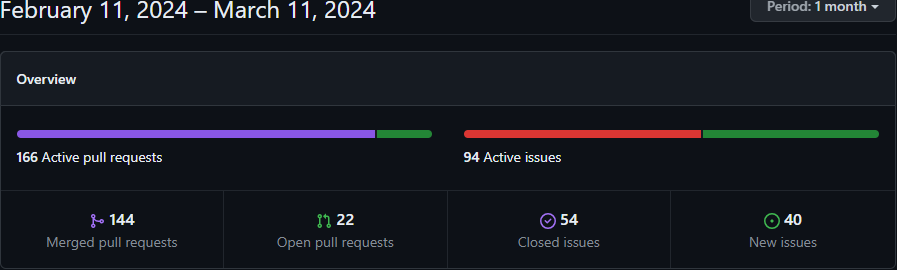
\includegraphics[width=0.75\linewidth]{source/implementation/evaluation/postgresql_ha_solutions/insights/cloudnativepg/pulse_cloudnative-pg_cloudnative-pg}
        \caption{CloudNativePG - Pulse}
        \label{fig:pulse_cloudnative-pg_cloudnative-pg}
    \end{figure}

    Der Code ist aber gut gepflegt, Code wird nicht nur regelmässig hinzugefügt, sondern auch entfernt.
    Auffällig ist, dass im April 2022 eine grosse Menge Code entfernt wurde:
    \begin{figure}[H]
        \centering
        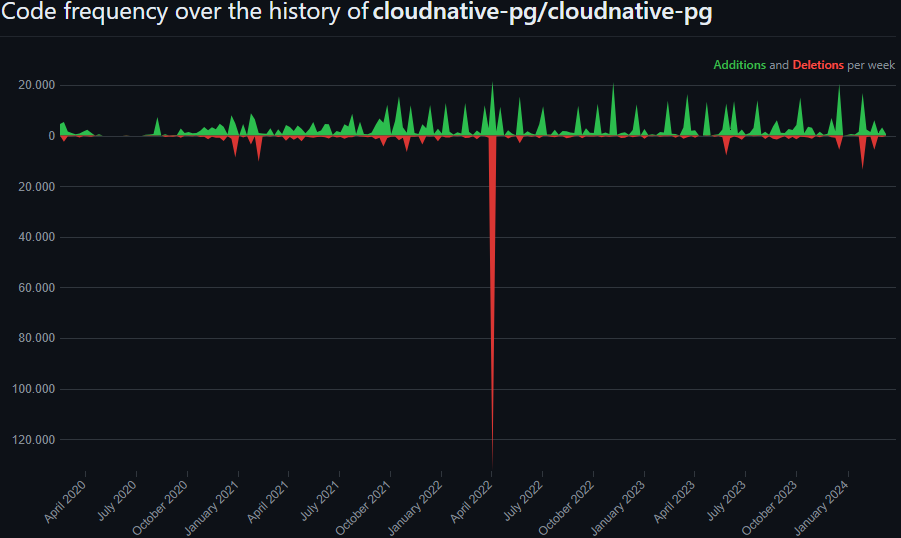
\includegraphics[width=0.75\linewidth]{source/implementation/evaluation/postgresql_ha_solutions/insights/cloudnativepg/code_frequency_cloudnative-pg_cloudnative-pg}
        \caption{CloudNativePG - Code Frequency}
        \label{fig:code_frequency_cloudnative-pg_cloudnative-pg}
    \end{figure}
\end{flushleft}
\clearpage
\begin{flushleft}
    Das Projekt hält die meisten Standards von GitHub ein:
    \begin{figure}[H]
        \centering
        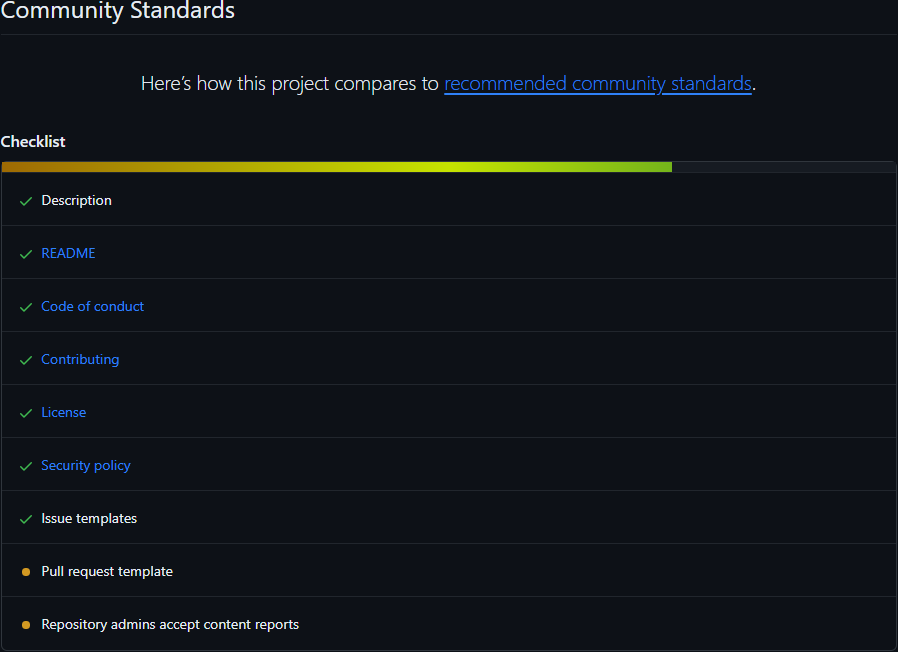
\includegraphics[width=0.75\linewidth]{source/implementation/evaluation/postgresql_ha_solutions/insights/cloudnativepg/community_standards}
        \caption{CloudNativePG - Community Standards}
        \label{fig:community_standards_cloudnativepg}
    \end{figure}
    Die Contributors committen zwar regelmässig auf das Projekt, allerdings fügen sie ungleich mehr dazu, als sie alten Code bereinigen.\\
    Das führt dann dazu, dass es zu grösseren Aufräumarbeiten kommt wie im April 2022.\\
    Es kann der Eindruck gewonnen werden, dass der Code wenig aufgeräumt wird und viel Ballast mit sich schleppt,\\
    was ein Sicherheitsrisiko darstellen kann:
    \begin{figure}[H]
        \centering
        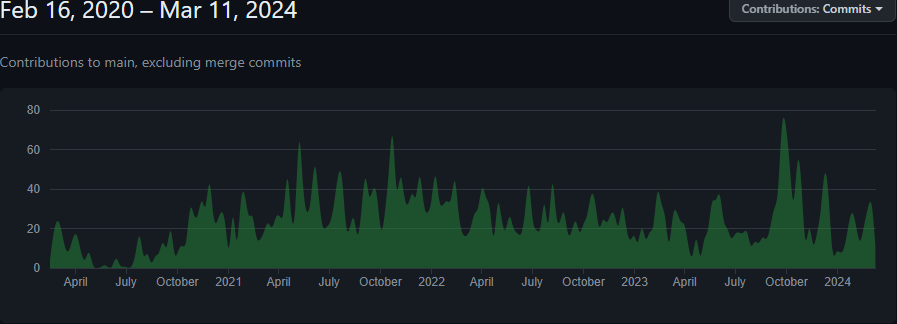
\includegraphics[width=0.75\linewidth]{source/implementation/evaluation/postgresql_ha_solutions/insights/cloudnativepg/contributors_commits_cloudnative-pg_cloudnative-pg}
        \caption{CloudNativePG - Contributors Commits}
        \label{fig:contributors_commits_cloudnative-pg_cloudnative-pg}
    \end{figure}
    \begin{figure}[H]
        \centering
        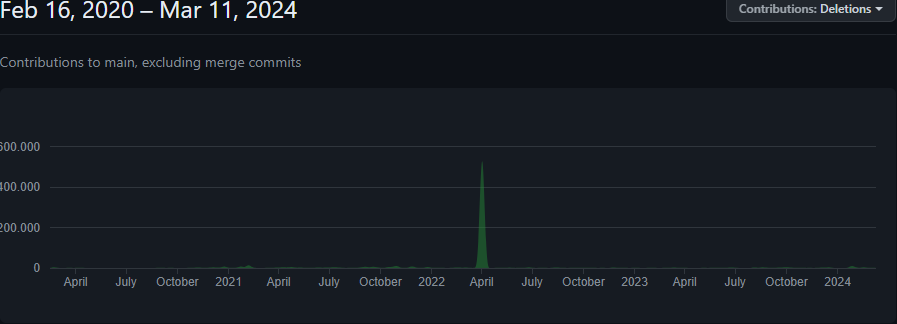
\includegraphics[width=0.75\linewidth]{source/implementation/evaluation/postgresql_ha_solutions/insights/cloudnativepg/contributors_deletations_cloudnative-pg_cloudnative-pg}
        \caption{CloudNativePG - Contributors Deletations}
        \label{fig:contributors_deletations_cloudnative-pg_cloudnative-pg}
    \end{figure}
    \begin{figure}[H]
        \centering
        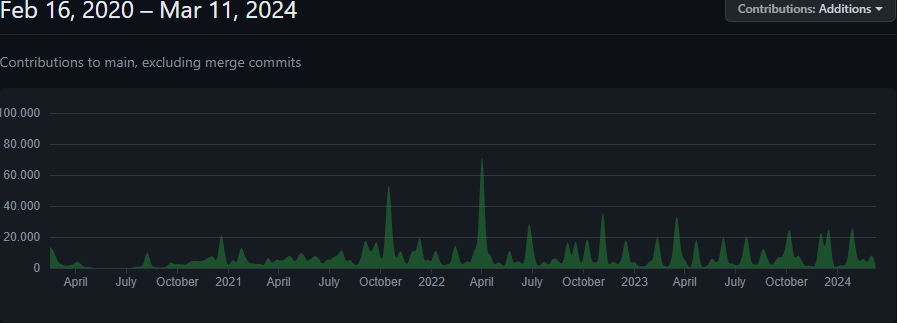
\includegraphics[width=0.75\linewidth]{source/implementation/evaluation/postgresql_ha_solutions/insights/cloudnativepg/contributors_additions_cloudnative-pg_cloudnative-pg}
        \caption{CloudNativePG - Contributors Additions}
        \label{fig:contributors_additions_cloudnative-pg_cloudnative-pg}
    \end{figure}
    Commits werden regelmässig abgesetzt, allerdings gibt es immer wieder gehäufte Commits.\\
    Oft um die Monatswechsel herum:
    \begin{figure}[H]
        \centering
        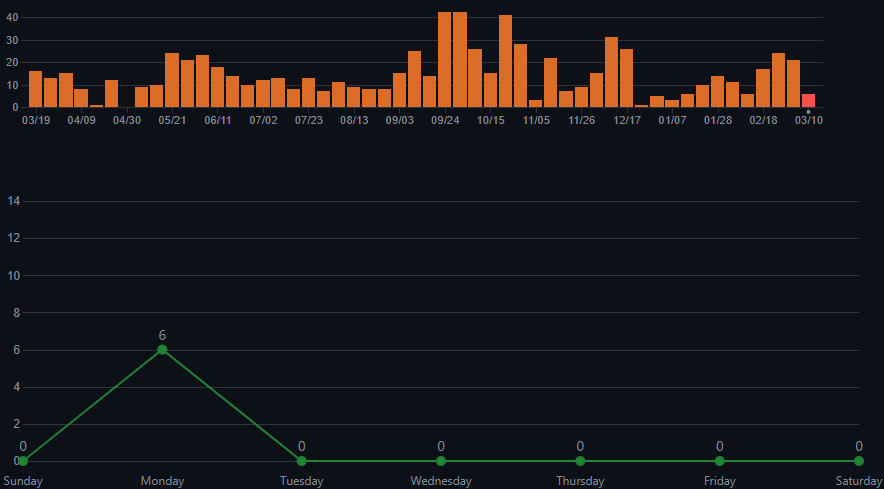
\includegraphics[width=0.75\linewidth]{source/implementation/evaluation/postgresql_ha_solutions/insights/cloudnativepg/commit_activity_cloudnative-pg_cloudnative-pg}
        \caption{CloudNativePG - Commit Activity}
        \label{fig:commit_activity_cloudnative-pg_cloudnative-pg}
    \end{figure}
\end{flushleft}
\clearpage
\begin{flushleft}
    Nebst dem Projekt cloudnative-pg der \guillemotleft© The CloudNativePG Contributors\guillemotright ist CloudNativePG-Gründer EDB noch immer ein grosser Contributor.
     \begin{figure}[H]
        \centering
        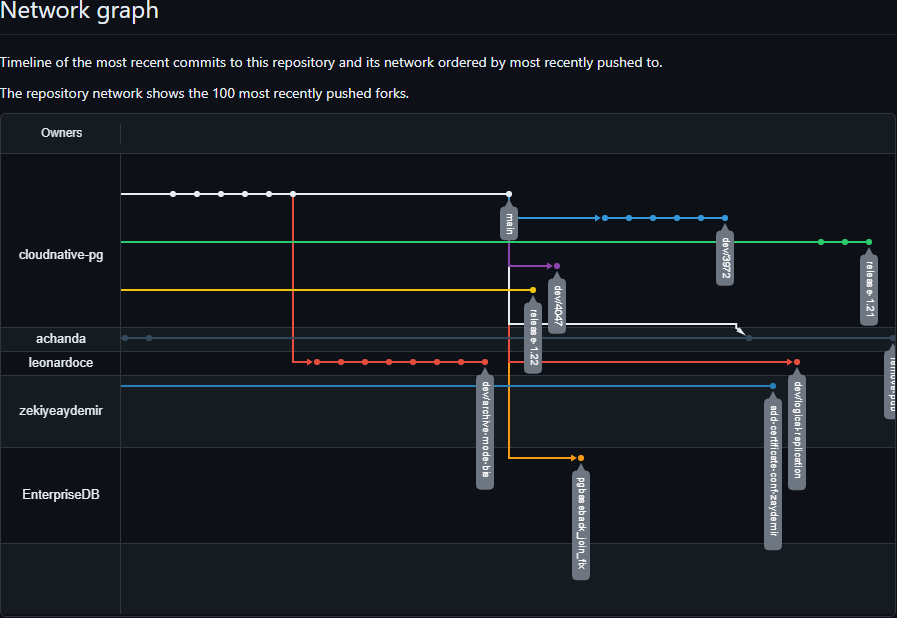
\includegraphics[width=0.75\linewidth]{source/implementation/evaluation/postgresql_ha_solutions/insights/cloudnativepg/network_graph_cloudnative-pg_cloudnative-pg}
        \caption{CloudNativePG - Network Graph}
        \label{fig:network_graph_cloudnative-pg_cloudnative-pg}
    \end{figure}
\end{flushleft}